\chapter{Literature review}

\section{Business Process Management}


\section{Business Process Mining}

While BPM covers the methods, techniques and tools that support the design, management and analysis of business processes ~\cite{van2003workflow}, data mining refers to the extraction of knowledge from data produced by a set of systems and processes. The combination of BPM and data mining has generated the new field of study known as process mining ~\cite{van2011process}, which aims to apply data mining techniques to data from the BPM lifecycle ~\cite{song2008trace} to extract in-depth insights from the event logs of workflow and BPM systems ~\cite{van2003workflow}.



Figure ~\ref{figure:BPMJ} introduces the components of process mining. Initially, the majority of process mining contributions focused on techniques for the discovery of processes (business process analysis), conformance checking (business process monitoring, business activity monitoring and process performance management) and various extensions ~\cite{song2008trace}, represented by the lower part of Figure 1. To enable these techniques, researchers also focused on log file preparation and mining algorithms ~\cite{weijters2006process}. Therefore, the first series of process mining papers primarily addressed the lower part of Figure ~\ref{figure:BPMJ}. Tiwari et al ~\cite{tiwari2008review} drew attention to the relationship between the process model and event logs by reviewing state-of-the-art process mining algorithms. Using 50 analyzed papers, they classified those that used process mining techniques and identified six practical challenges. The process mining manifesto ~\cite{van2012process} renewed these challenges and identified 11 challenges. While Tiwari et al. ~\cite{tiwari2008review} primarily addressed problematic log file preparation (e.g. noise, hidden tasks, duplicate tasks, etc.), the challenges of the process mining manifesto have a broader perspective covering the application and representation of process mining, e.g., balancing quality criteria such as fitness, simplicity, precision and generalization, cross-organizational mining and operational support.


\begin{figure}[!htb]
    \centering 
    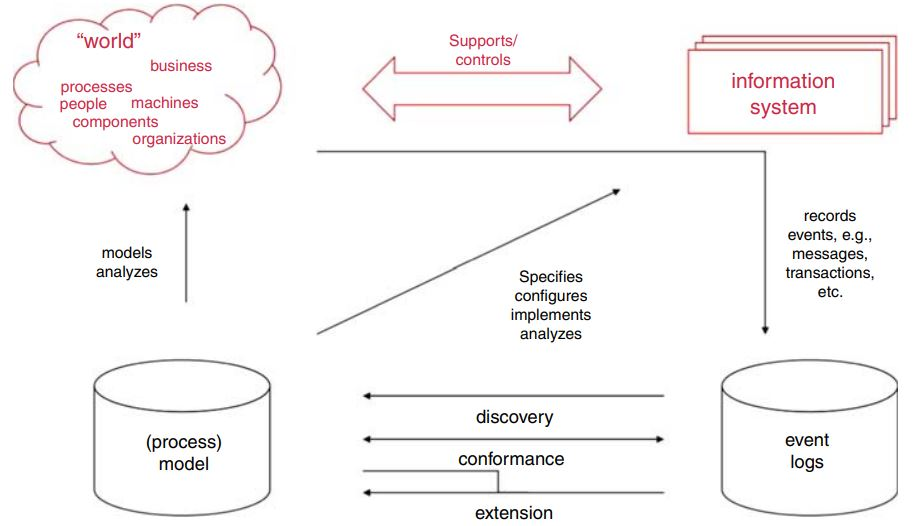
\includegraphics[scale=0.7]{resource/BPMJ.JPG}
    \caption{source: Adpoted from Van der Aalst ~\cite{van2011process}}
    \label{figure:BPMJ}
\end{figure}



The study of event logs and how they are extracted from ISs (right part of Figure 1) are addressed by Rozinat and van der~\cite{rozinat2006decision}, de Medeiros and Günther ~\cite{de2005process} and Adriansyah et al. ~\cite{adriansyah2011conformance}. In these studies, the conformance of event logs and real world or reference models is assessed. Other authors address the use of process models in real-world accounting (left part of Figure 1), e.g., for forced behavior ~\cite{wen2009novel}, concept drift ~\cite{engel2014case} and security ~\cite{van2005process}. Finally, Maruster et al. ~\cite{muarucster2006rule} discuss noise cancellation in event logs.

Later research focuses more on the upper-red part of Figure 1, i.e., the relationship between the “world” and ISs. While Turner et al. (2012) provide an overview of the process mining tools available in the UK market, other studies address either the combination of process mining with other technologies (e.g. artificial neural networks, support vector machines) (Maita et al., 2015) or a specific application area (e.g. healthcare) (Rojas et al., 2016; Yang and Su, 2014). Our study follows Rojas et al.’s path and addresses the relationship between the “world,” more specifically, “organizations,” and IS, which is marked in red in Figure 1. Similar to the most recent reviews (Kurniati et al., 2016; Maita et al., 2015; Rojas et al., 2016), we follow a systematic literature review approach. However, we adopt a broader scope to analyze empirical studies on process mining that is not limited to a specific market or application area.




